% This work is licensed under the Creative Commons
% Attribution-NonCommercial-ShareAlike 4.0 International License. To view a copy
% of this license, visit http://creativecommons.org/licenses/by-nc-sa/4.0/ or
% send a letter to Creative Commons, PO Box 1866, Mountain View, CA 94042, USA.
% vim: set noexpandtab:

% the following tikz picture was auto-generated by:
% https://www.mathcha.io/editor

\tikzset{every picture/.style={line width=0.75pt}} %set default line width to 0.75pt        

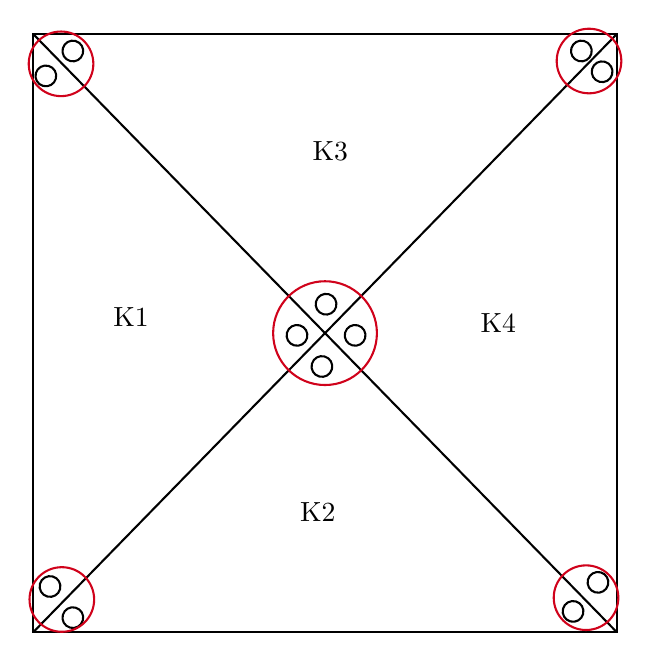
\begin{tikzpicture}[x=0.75pt,y=0.75pt,yscale=-1,xscale=1]
%uncomment if require: \path (0,300); %set diagram left start at 0, and has height of 300

%Shape: Rectangle [id:dp14549454055533384] 
\draw   (64,2.93) -- (345,2.93) -- (345,290.93) -- (64,290.93) -- cycle ;
%Straight Lines [id:da9627683453327494] 
\draw    (64,2.93) -- (345,290.93) ;


%Straight Lines [id:da9434997856090799] 
\draw    (345,2.93) -- (64,290.93) ;


%Straight Lines [id:da169571524037062] 
\draw    (100,130) ;


%Shape: Circle [id:dp7836721006446373] 
\draw   (186.18,146.69) .. controls (186.9,144.02) and (189.65,142.45) .. (192.31,143.18) .. controls (194.98,143.9) and (196.55,146.65) .. (195.82,149.31) .. controls (195.1,151.98) and (192.35,153.55) .. (189.69,152.82) .. controls (187.02,152.1) and (185.45,149.35) .. (186.18,146.69) -- cycle ;
%Shape: Circle [id:dp7887685534943322] 
\draw   (214.18,146.69) .. controls (214.9,144.02) and (217.65,142.45) .. (220.31,143.18) .. controls (222.98,143.9) and (224.55,146.65) .. (223.82,149.31) .. controls (223.1,151.98) and (220.35,153.55) .. (217.69,152.82) .. controls (215.02,152.1) and (213.45,149.35) .. (214.18,146.69) -- cycle ;
%Shape: Circle [id:dp792561043036806] 
\draw   (198.18,161.69) .. controls (198.9,159.02) and (201.65,157.45) .. (204.31,158.18) .. controls (206.98,158.9) and (208.55,161.65) .. (207.82,164.31) .. controls (207.1,166.98) and (204.35,168.55) .. (201.69,167.82) .. controls (199.02,167.1) and (197.45,164.35) .. (198.18,161.69) -- cycle ;
%Shape: Circle [id:dp5381851880499974] 
\draw   (200.18,131.69) .. controls (200.9,129.02) and (203.65,127.45) .. (206.31,128.18) .. controls (208.98,128.9) and (210.55,131.65) .. (209.82,134.31) .. controls (209.1,136.98) and (206.35,138.55) .. (203.69,137.82) .. controls (201.02,137.1) and (199.45,134.35) .. (200.18,131.69) -- cycle ;
%Shape: Circle [id:dp44002878595191575] 
\draw   (78.18,282.69) .. controls (78.9,280.02) and (81.65,278.45) .. (84.31,279.18) .. controls (86.98,279.9) and (88.55,282.65) .. (87.82,285.31) .. controls (87.1,287.98) and (84.35,289.55) .. (81.69,288.82) .. controls (79.02,288.1) and (77.45,285.35) .. (78.18,282.69) -- cycle ;
%Shape: Circle [id:dp42740284154555863] 
\draw   (67.18,267.69) .. controls (67.9,265.02) and (70.65,263.45) .. (73.31,264.18) .. controls (75.98,264.9) and (77.55,267.65) .. (76.82,270.31) .. controls (76.1,272.98) and (73.35,274.55) .. (70.69,273.82) .. controls (68.02,273.1) and (66.45,270.35) .. (67.18,267.69) -- cycle ;
%Shape: Circle [id:dp6205100758907591] 
\draw   (319.18,279.69) .. controls (319.9,277.02) and (322.65,275.45) .. (325.31,276.18) .. controls (327.98,276.9) and (329.55,279.65) .. (328.82,282.31) .. controls (328.1,284.98) and (325.35,286.55) .. (322.69,285.82) .. controls (320.02,285.1) and (318.45,282.35) .. (319.18,279.69) -- cycle ;
%Shape: Circle [id:dp12003747556472932] 
\draw   (331.18,265.69) .. controls (331.9,263.02) and (334.65,261.45) .. (337.31,262.18) .. controls (339.98,262.9) and (341.55,265.65) .. (340.82,268.31) .. controls (340.1,270.98) and (337.35,272.55) .. (334.69,271.82) .. controls (332.02,271.1) and (330.45,268.35) .. (331.18,265.69) -- cycle ;
%Shape: Circle [id:dp3476040811313178] 
\draw   (333.18,19.69) .. controls (333.9,17.02) and (336.65,15.45) .. (339.31,16.18) .. controls (341.98,16.9) and (343.55,19.65) .. (342.82,22.31) .. controls (342.1,24.98) and (339.35,26.55) .. (336.69,25.82) .. controls (334.02,25.1) and (332.45,22.35) .. (333.18,19.69) -- cycle ;
%Shape: Circle [id:dp21135819336466033] 
\draw   (323.18,9.69) .. controls (323.9,7.02) and (326.65,5.45) .. (329.31,6.18) .. controls (331.98,6.9) and (333.55,9.65) .. (332.82,12.31) .. controls (332.1,14.98) and (329.35,16.55) .. (326.69,15.82) .. controls (324.02,15.1) and (322.45,12.35) .. (323.18,9.69) -- cycle ;
%Shape: Circle [id:dp08585658948454522] 
\draw   (78.18,9.69) .. controls (78.9,7.02) and (81.65,5.45) .. (84.31,6.18) .. controls (86.98,6.9) and (88.55,9.65) .. (87.82,12.31) .. controls (87.1,14.98) and (84.35,16.55) .. (81.69,15.82) .. controls (79.02,15.1) and (77.45,12.35) .. (78.18,9.69) -- cycle ;
%Shape: Circle [id:dp07079948382140533] 
\draw   (65.18,21.69) .. controls (65.9,19.02) and (68.65,17.45) .. (71.31,18.18) .. controls (73.98,18.9) and (75.55,21.65) .. (74.82,24.31) .. controls (74.1,26.98) and (71.35,28.55) .. (68.69,27.82) .. controls (66.02,27.1) and (64.45,24.35) .. (65.18,21.69) -- cycle ;
%Shape: Circle [id:dp6214173079072771] 
\draw  [color={rgb, 255:red, 208; green, 2; blue, 27 }  ,draw opacity=1 ] (179.5,146.93) .. controls (179.5,133.13) and (190.69,121.93) .. (204.5,121.93) .. controls (218.31,121.93) and (229.5,133.13) .. (229.5,146.93) .. controls (229.5,160.74) and (218.31,171.93) .. (204.5,171.93) .. controls (190.69,171.93) and (179.5,160.74) .. (179.5,146.93) -- cycle ;
%Shape: Circle [id:dp8527921748422009] 
\draw  [color={rgb, 255:red, 208; green, 2; blue, 27 }  ,draw opacity=1 ] (314.69,274.39) .. controls (314.69,265.8) and (321.66,258.82) .. (330.26,258.82) .. controls (338.85,258.82) and (345.82,265.8) .. (345.82,274.39) .. controls (345.82,282.99) and (338.85,289.96) .. (330.26,289.96) .. controls (321.66,289.96) and (314.69,282.99) .. (314.69,274.39) -- cycle ;
%Shape: Circle [id:dp9683122242620462] 
\draw  [color={rgb, 255:red, 208; green, 2; blue, 27 }  ,draw opacity=1 ] (316.12,15.82) .. controls (316.12,7.23) and (323.09,0.26) .. (331.69,0.26) .. controls (340.29,0.26) and (347.26,7.23) .. (347.26,15.82) .. controls (347.26,24.42) and (340.29,31.39) .. (331.69,31.39) .. controls (323.09,31.39) and (316.12,24.42) .. (316.12,15.82) -- cycle ;
%Shape: Circle [id:dp7791705596437565] 
\draw  [color={rgb, 255:red, 208; green, 2; blue, 27 }  ,draw opacity=1 ] (61.74,17.18) .. controls (61.74,8.58) and (68.71,1.61) .. (77.31,1.61) .. controls (85.91,1.61) and (92.88,8.58) .. (92.88,17.18) .. controls (92.88,25.77) and (85.91,32.74) .. (77.31,32.74) .. controls (68.71,32.74) and (61.74,25.77) .. (61.74,17.18) -- cycle ;
%Shape: Circle [id:dp5325582065155569] 
\draw  [color={rgb, 255:red, 208; green, 2; blue, 27 }  ,draw opacity=1 ] (62.12,275.26) .. controls (62.12,266.66) and (69.09,259.69) .. (77.69,259.69) .. controls (86.29,259.69) and (93.26,266.66) .. (93.26,275.26) .. controls (93.26,283.85) and (86.29,290.82) .. (77.69,290.82) .. controls (69.09,290.82) and (62.12,283.85) .. (62.12,275.26) -- cycle ;

% Text Node
\draw (111,139) node  [align=left] {K1};
% Text Node
\draw (201,233) node  [align=left] {K2};
% Text Node
\draw (207,59) node  [align=left] {K3};
% Text Node
\draw (288,142) node  [align=left] {K4};


\end{tikzpicture}













